\documentclass{scrartcl}
\usepackage{hyperref}
\usepackage{graphicx}
\usepackage{subfig}

\graphicspath{{./images/}}

\title{Explainable SVM}
\subtitle{Online Visualizations for Teaching}

% FIXME emails look weird?
\author{
  Hendrik Pfaff, Luca Jordan, Lukas Atkinson, Yasemin Er
  \\
  {\normalsize\ttfamily \{hendrik.pfaff,gian.jordan,atkinson,yasemin-\}@stud.fra-uas.de}
}

\date{Summer Term 2020}

\publishers{Frankfurt University of Applied Sciences}

\subject{Project Documentation}

\begin{document}
\maketitle

\section{Introduction}

In order to teach algorithms, interactive visualizations can be a powerful tool.
We therefore developed an interactive, web-based tool
to explain how Support Vector Machines (SVM) work.

\section{Support Vector Machines}

\subsection*{SVM Parameters}

\subsubsection*{Epsilon $\epsilon$}
Intuitively, the $\epsilon$ parameter defines how far the influence of a single training example reaches, with low values meaning ‘far’ and high values meaning ‘close’. The $\epsilon$ parameters can be seen as the inverse of the radius of influence of samples selected by the model as support vectors. When $\epsilon$ is very small, the model is too constrained and cannot capture the complexity or 'shape' of the data. The region of influence of any selected support vector would include the whole training set. The resulting model will behave similarly to a linear model with a set of hyperplanes that separate the centers of high density of any pair of two classes. 

\begin{figure}%
	\centering
	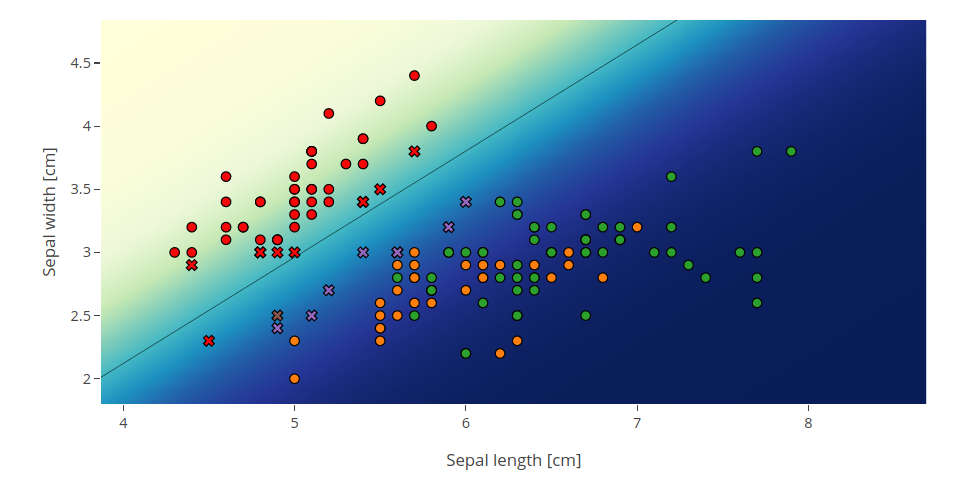
\includegraphics[height=8cm]{IrisLin001_1}
	\caption{Small Epsilon (0.001) in combination with small C shifts the decision boundary evenly between the two classes that are to be separated. The support vectors are displayed as crosses. Based on these vectors, the boundary is drawn.}
	\label{fig:example}%
\end{figure}

\begin{figure}%
	\centering
	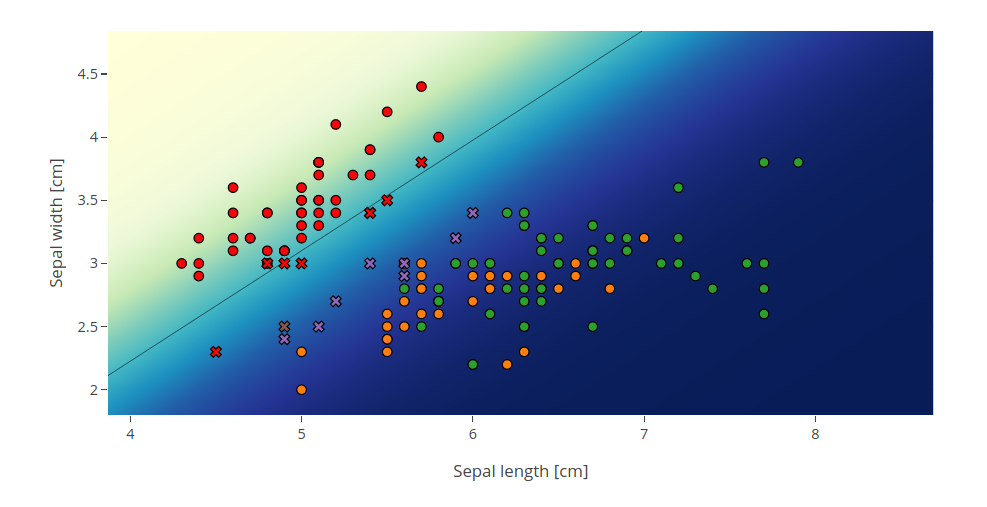
\includegraphics[height=8cm]{IrisLin51}
	\caption{Large Epsilon (0.5) shifts the decision boundary too far into the red cluster. This is due to the parameter Epsilon regulating how much influence each datapoint is assigned to, to move the decision boundary. In this case, the choice of parameters is not optimal, nevertheless most datapoints from the red cluster are classified correctly.}%
	\label{fig:example}%
\end{figure}
\newpage
\subsubsection*{C}
The C parameter trades off correct classification of training examples against maximization of the decision function’s margin. For larger values of C, a smaller margin will be accepted if the decision function is better at classifying all training points correctly. A lower C will encourage a larger margin, therefore a simpler decision function, at the cost of training accuracy. In other words: C behaves as a regularization parameter in the SVM. As you can see when applying larger values for C, the support vectors move farther away from the decision boundary. Support vectors are displayed as X's. 

\begin{itemize}
	\item \textbf{Small C} makes the constraints easy to ignore which leads to a large margin
	\item \textbf{Large C} allows the constraints hard to be ignored which leads to a small margin
	\item For \textbf{C = inf}, all the constraints are enforced.
\end{itemize}

\begin{figure}[h!]%
	\centering
	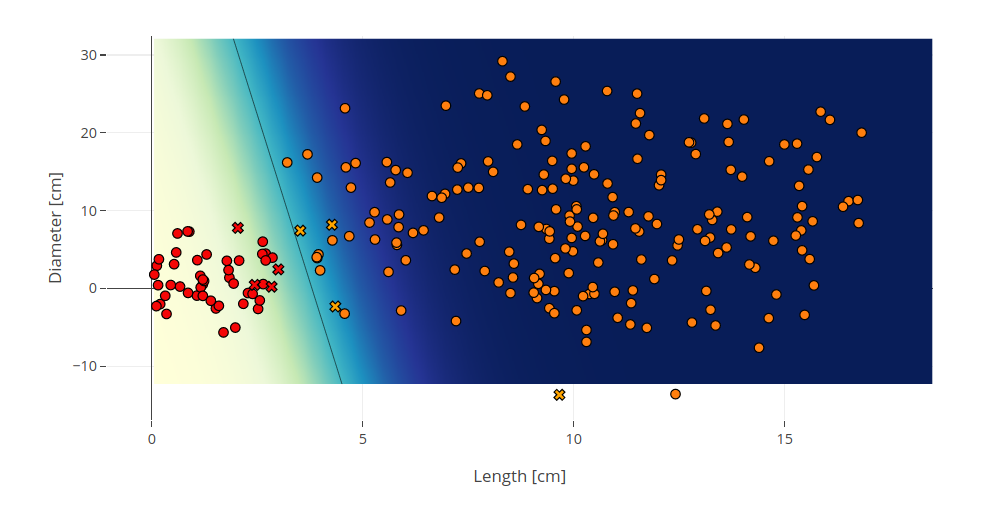
\includegraphics[height=8cm]{SalmonLin75_1}
	\caption{When picking a small value (~1) for the C parameter in combination with a large Epsilon (0.75) the decision boundary is placed correctly balanced between the two classes.}
	\label{fig:example}%
\end{figure}

\begin{figure}[h!]%
	\centering
	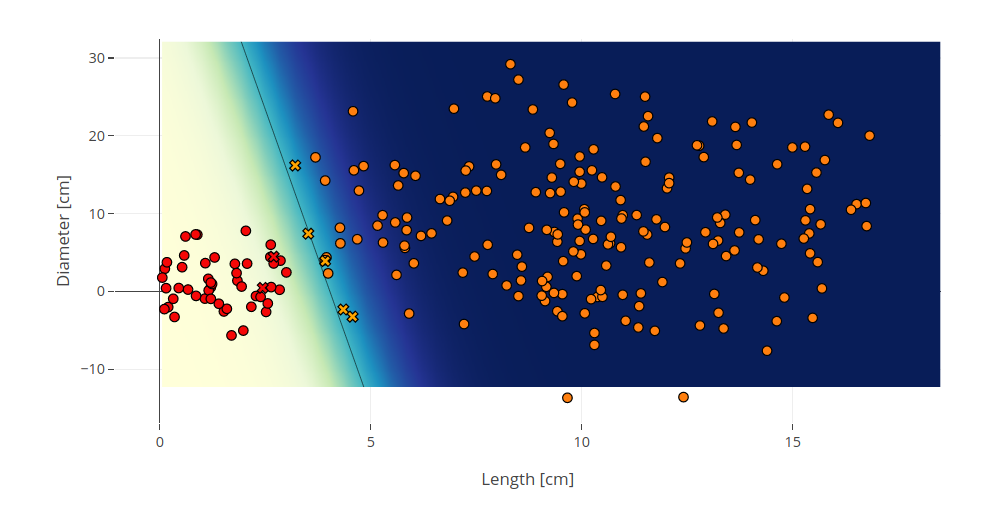
\includegraphics[height=8cm]{SalmonLin75_10k}
	\caption{With an increasingly large C parameter (C=10.000) the decision boundary may move too much towards one of the class clusters. In this example, the prediction of the orange datapoints is still correct, yet it is clearly visible that some datapoints are dangerously close to the decision boundary.}%
	\label{fig:example}%
\end{figure}



% TODO: provide some mathematical background
\newpage
\section{Installation}

The visualizations are implemented in client-side JavaScript,
so implementation is simple:
the project files just have to be served via an HTTP server
and opened in any modern browser.
There are no server-side programs that have to be installed.

For local use, Python's built-in web server is a convenient choice:

\begin{enumerate}
\item start the server with \verb|python3 -m http.server -b localhost 4321|
\item open the start page in the browser: \url{http://localhost:4321/views/}
\end{enumerate}

While the user-accessible pages are under \verb|/views/|,
necessary resources are served under
\verb|/data/|, \verb|/css/|, and \verb|/js/|.

A live version of the project can also be accessed at
\url{https://luckyviking.github.io/WebViz/views/}.



\section{Implemented Views}

The primary tool is provided under \verb|/views/plotly.html|.
Other tools were used for debugging or tried out alternative approaches:

\begin{itemize}
\item \verb|/views/scatterplot.html|
\item \verb|/views/different_datasets.html|
\item \verb|/views/iris_shapes.html|
\item \verb|/views/gui.html|
\item \verb|/views/plotly.html|
\end{itemize}

\subsection*{Visualization}

%\subsubsection*{Used Tools and Libraries}
Starting the project, the plan was to do the visualization using d3.js, which is one of the most used visualization libraries for Javascript with over 50k related repositories on Github. It enhances the user to visualize almost any given dataset by providing the ability to assemble custom tailored plots and visualizations using many different modules that can be combined to produce individual and interactive visualizations. Unfortunately, as it often tends to be the case for libraries that offer a lot of individuality, producing contour or line plots using d3.js requires quite some effort to get started with, as the amount of different possibilities is very large. So as a matter of fact, that the project was set to 6 months, the decision was made to make use of another data visualization library, Plotly, that offers many standard features that work out of the box and can be combined with different data.
Plotly is at least as well known as d3.js, being a widely used plotting library, that is available for different programming languages such as Python, R, Javascript. Plotly.js offers many possibilities to visualize different kinds of plots which can be integrated into websites via Javascript, CSS and HTML. Comparing d3.js with plotly.js the team came to the conclusion, that d3.js offers much more freedom to produce very custom visualizations, while plotly.js offers the most common types of plots for data visualization. Therefore, we decided to go with usability rather than adaptability.
Furthermore, other libraries such as jQuery, Ajax, Bootstrap and Mathjax enable the full functionality of Javascript powered Websites.


To visualize the behavior of an SVM on different kernels, datasets and parameters several plotting features from Plotly were combined into a single plot. 
Firstly, the data points contained in the available datasets have to be visualized using a scatter plot, which plots the data points in accordance to their feature values in a 2D coordinate system, where x- and y-axis correspond to two features of the data set. 
For example plotting the Iris dataset, the x-axis could correspond to Sepa length and the y-axis to Sepal width. Subsequently, the data points can be drawn into the coordinate system. Simultaneously, the different data points may be shown in different colors or shapes according to their label which is also the desired output of the SVM.

For visualizing the decision boundary of the SVM a Contour plot was used. The corresponding contour results from the SVM predicting the labels for different data points of the z-array. The z-array yields the entire co-domain of the two features from the training set and is arranged in an array. The x-axis is ranging from Min(Feature 1) to Max(Feature 1) and the y-axis from Min(Feature 2) to Max(Feature 2). All the resulting data points in the z-array are passed to the pre-trained SVM for predicting their label. The output of the SVM is another array with the same shape as the z-array. The resulting array is further smoothed using the Sigmoid function, which maps all values to between 0 and 1, where 0 corresponds to one class and 1 to the other. 
At this point, a two leveled contour plot can be used with the resulting z-array  to visualize the decision boundary of the SVM. The contour plot is further expanded with a heatmap, that visualizes the decision margins and the two classes in different colors.
Another Scatterplot is added to also display the support vectors, as their positions change when the parameters of the SVM are changed, this is an important point to explain the behavior of an SVM to students.


\section{User Manual}

\section{Challenges}

\section{Conclusion}

\end{document}